\documentclass[10pt]{beamer}
\usetheme[
%%% option passed to the outer theme
%    progressstyle=fixedCircCnt,   % fixedCircCnt, movingCircCnt (moving is deault)
  ]{Feather}
  
% If you want to change the colors of the various elements in the theme, edit and uncomment the following lines

% Change the bar colors:
%\setbeamercolor{Feather}{fg=red!20,bg=red}

% Change the color of the structural elements:
%\setbeamercolor{structure}{fg=red}

% Change the frame title text color:
%\setbeamercolor{frametitle}{fg=blue}

% Change the normal text color background:
%\setbeamercolor{normal text}{fg=black,bg=gray!10}

%-------------------------------------------------------
% INCLUDE PACKAGES
%-------------------------------------------------------

\usepackage[utf8]{inputenc}
\usepackage[english]{babel}
\usepackage[T1]{fontenc}
\usepackage{helvet}
\usepackage{caption}
\usepackage{subcaption}
\usepackage{graphicx} % Allows including images
%-------------------------------------------------------
% DEFFINING AND REDEFINING COMMANDS
%-------------------------------------------------------

% colored hyperlinks
\newcommand{\chref}[2]{
  \href{#1}{{\usebeamercolor[bg]{Feather}#2}}
}

%-------------------------------------------------------
% INFORMATION IN THE TITLE PAGE
%-------------------------------------------------------

\title[] % [] is optional - is placed on the bottom of the sidebar on every slide
{ % is placed on the title page
      \textbf{The Laplacian matrix and Applications}
}

\subtitle[]
{
     
}

\author[Alice Nanyanzi]
{     Alice Nanyanzi \\
      %{\ttfamily alicenanyanzi@aims.ac.za} 
}

\institute[]
{
      AIMS - STELLENBOSCH UNIVERSITY\\
      South Africa
  
  %there must be an empty line above this line - otherwise some unwanted space is added between the university and the country (I do not know why;( )
}

\date{\today}

%-------------------------------------------------------
% THE BODY OF THE PRESENTATION
%-------------------------------------------------------

\begin{document}

%-------------------------------------------------------
% THE TITLEPAGE
%-------------------------------------------------------

{\1% % this is the name of the PDF file for the background
\begin{frame}[plain,noframenumbering] % the plain option removes the header from the title page, noframenumbering removes the numbering of this frame only
  \titlepage % call the title page information from above
\end{frame}}


\begin{frame}{Content}{}
\tableofcontents
\end{frame}
\section{Complex systems \& Complex Networks} 
\begin{frame}{Complex Systems; Complex Network/Large graph Approach}
	
	\begin{figure}[!h]
		\centering
		\includegraphics[width=0.75\textwidth]{images/abstract-diagram.pdf}
		\caption{}
		%\label{stardifn-graph}
	\end{figure}
	
\end{frame}

%------------------------------------------------
\section{Overview of Networks}
\begin{frame}
	\frametitle{Introduction to Networks}
	
	\only<1->{\begin{block}{Intuition of Networks}
			Whenever one mentions the word 'network', one normally thinks of an interconnection of items or things.
	\end{block} }
	
	\vspace{0.5cm}
	
	\only<2>{\begin{block}{Formal Definition}
			A network, $G$, is a pair $(V,E)$. Where $V$ is the set of vertices (nodes) of $G$ and $E$ is the set of edges (links) of $G$. (Estrada \& Knight).\\
			Categories of networks include simple networks, directed networks, undirected networks, weighted networks, etc  (Estrada, 2015)
	\end{block}}
	
	
\end{frame}

\begin{frame}
	\frametitle{Real-world Networks}
	\begin{figure}[!h]
		%\centering
		\begin{subfigure}[b]{0.3\textwidth}
			\includegraphics[width=\textwidth]{images/Steve-Jurvetson.jpg}
			\caption{Internet}
			%\label{stardifn-graph}
		\end{subfigure}\qquad
		\begin{subfigure}[b]{0.3\textwidth}
			\includegraphics[width= \textwidth]{images/yeastprotein-protein-interactions.jpeg}
			\caption{Protein-Protein }
			%\label{stardifn-plot}
		\end{subfigure}\\
		\begin{subfigure}[b]{0.3\textwidth}
			\includegraphics[width=\textwidth]{images/food-web-2.png}
			\caption{Food web}
			%\label{regdifn-graph}
		\end{subfigure}~
		\begin{subfigure}[b]{0.3\textwidth}
			\includegraphics[width= \textwidth]{images/citation.jpg}
			\caption{Citation network}
			%\label{regdifn-plot}
		\end{subfigure}
	\end{figure}
	Source: www.wikipedia.com
\end{frame}

\section{Laplacian Matrix}
\begin{frame}
	\frametitle{Laplacian Matrix}
	\begin{block}{Definition}
		Consider a simple undirected network, the Laplacian matrix $L$ is the difference between the Degree matrix $D$ and Adjacency matrix $A$ i.e\\
		$L= D-A$. The entries of $L$ are given as\\
		\vspace{0.5 cm}
		$
		L_{i,j} = \begin{cases}
		k_i & \text{ if }  i=j\\
		-1  & \text{if } i \neq j \text{ and } i \text{ is adjacent to } j \\
		0 & \text{otherwise},
		\end{cases}
		$\\
		where $k_i$ denotes the degree of node $i$ (Estrada, 2011).
	\end{block}
\end{frame}

\begin{frame}{Spectrum of the Laplacian Matrix}
	\only<1->{\begin{block}{Spectrum}
			Spectrum of a matrix is a set eigenvalues and their multiplicities. Let $\lambda_i$ denote the eigenvalues of the Laplacian matrix. Considering the nondecreasing order: $\lambda_n  \geq \lambda_{n-1} \geq  \cdots \geq \lambda_2 \geq \lambda_1 =0 $
	\end{block}}
	
	\only<2> {\begin{block}{Insights from spectrum}
			\begin{itemize}
				\item The multiplicity of $0$ as an eigenvalue of $\mathbf{L}$ is equal to the number of connected components in the network.
				\item  A network, G, is connected if its second smallest eigenvalue is nonzero. That is, $\lambda_2> 0$ if and only if $G$ is connected. The eigenvalue $\lambda_2$ is thus called the algebraic connectivity of a network, $a(G)$ (Estrada, 2011).
			\end{itemize}
	\end{block}}
	
\end{frame}
\begin{frame} {Applications of Laplacian Matrix}
	\begin{itemize}
		\item Centrality measure
		\item Diffusion on network
		\item Consensus in multi-agent systems
		\item Synchronization  
	\end{itemize}
\end{frame}
\begin{frame}{Centrality Measures}
	In networks, centrality is the measure how important/central a node is, in the network (Newman, 2010). There exists various measures such as:
	\begin{itemize}[<+(1)->]
		\item \textcolor{red}{Degree centrality}: Power through links
		\item  \textcolor{red}{Closeness centrality}: Power through proximity to others
		\item  \textcolor{red}{Betweenness centrality}: Ability to act as a bridge
		\item  \textcolor{red}{Eigenvector centrality}: Improvement in degree centrality
		\item  \textcolor{red}{Subgraph centrality}: Participation of a node in subgraphs in network
		\item  \textcolor{red}{Laplacian centrality} : Impact of deactivation of a node from the network.
	\end{itemize} 
\end{frame}
\subsection{Laplacian Centrality}
\begin{frame}{Laplacian Centrality}
	\begin{itemize}
		\item Work presented is based on the paper: Laplacian centrality: A new centrality measure for weighted networks  by Qi et al., 2012.
	\end{itemize}
	\vspace{0.2cm}
	\begin{block}{Motivation}
		\begin{itemize}
			\item The growing need for centrality measures for weighted networks since these networks contain rich information (Qi et al., 2012).
			\vspace{0.2cm}
			\pause
			\item  Standard centrality measures (degree, closeness, betweenness) have been extended to cater for weighted networks, however, these measures either capture the local or global characterisation of networks (T.Opsahl '2009, Newman '2001, A.Barrat '2004, U.Brandes '2001). 
			\vspace{0.2cm}
			\pause
			\item The Laplacian centrality is a measure between local and global (i.e intermediate) characterisation of the centrality of a node.
		\end{itemize}
	\end{block}
\end{frame}

\begin{frame}{Laplacian Centrality Cont....}
	\begin{block}{Laplacian Energy of a Network}
		The importance of a node is determined by the ability of the network to respond to the deactivation  of the node from the network. The response is quantified by the relative drop in Laplacian energy ($E_{L}$) of the network (Qi et al., 2012).
		\vspace{0.4cm}
		
		\begin{equation}
		E_L(G) = \sum_{i=1}^n \lambda_i ^2 = \sum_{i=1}^n x_i^2 + 2 \sum_{i<j} w_{i,j}^2,
		\end{equation}
		where $x_i's$ are vertex sums and $w_{ij}$ are weights of edges between vertices $i$ and $j$ (Qi et al., 2012).
	\end{block}
\end{frame}

\begin{frame}{Mathematical Formulation of Laplacian Centrality}
	Mathematically, Laplacian centrality for a node $i$ in network $G$ is given by (Qi et al., 2012) \\
	\vspace{0.2cm}
	\begin{equation}
	C_L(v_i,G) = \frac{(\Delta E)_i}{E_L(G)} = \frac{E_L(G) - E_L(G_i)}{E_L(G)},
	\label{lapcent}
	\end{equation}
	where \\
	$E_L(G)$ - Laplacian energy of network $G$.\\
	$E_L(G_i)$ - Laplacian energy of network $G$ on removal of node $i$
\end{frame}

\begin{frame}{Graph Theoretical Interpretation of Laplacian Centrality}
	Expressing Equation \ref*{lapcent} in terms of $2$-walks of the node $i$ gives
	\begin{equation}
	(\Delta E)_i = 2\cdot NW_{2} ^M(v_i) + 2 \cdot NW_{2} ^E(v_i) + 4 \cdot NW_{2} ^C(v_i), 
	\end{equation}
	\vspace{0.3cm}
	where 
	$NW_{2} ^C(v_i)$, $NW_{2} ^E(v_i)$, and $NW_{2} ^M(v_i)$ are closed $2$-walks containing vertex $v_i$, non-closed $2$-walks with vertex $v_i$ as one of the end points and non-closed $2$-walks with vertex $v_i$ as the middle point
	(Qi et al., 2012).
	
	\begin{figure}[!h]
		\centering
		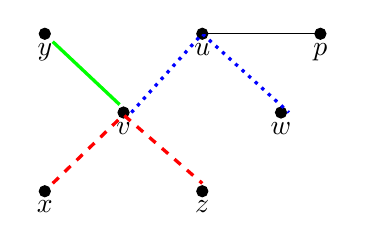
\begin{tikzpicture}
		\filldraw
		(0,0) circle (2pt) node[align=left, below] {$x$} 
		(1,1) circle (2pt) node[align=center, below] {$v$}    
		(0,2) circle (2pt) node[align=right,  below] {$y$}
		(2,2) circle (2pt) node[align=right,  below] {$u$}
		(2,0) circle (2pt) node[align=center, below] {$z$}  
		(3,1) circle (2pt) node[align=right,  below] {$w$}
		(3.5,2) circle (2pt) node[align=right,  below] {$p$};
		\draw[red, dashed, very thick] (0.1,0.1) -- (1.0,0.97) -- (2.0,0.1);	
		\draw[blue,dotted, very thick] (1.1,1.0) -- (2.0,2.0) -- (3.1,1.0);
		\draw[green,solid, very thick] (0.95,1.1) -- (0.1,1.9) -- (0.95,1.1);	
		\draw[] (2,2) -- (3.5,2);		
		\end{tikzpicture}
		\caption{$2$-walks at node $v$}
	\end{figure}
	
\end{frame}

\begin{frame}{Application to real-world networks}
	\begin{block}{Zachary's Karate Network}
		\begin{itemize}
			\item \textbf{The Zachary's Karate Network} was created from a dataset formed by observation of $34$ members of a karate club over two years. Misunderstandings within the group led to a split into two groups, one led by the Administrator ($1$) and the other by the instructor ($34$).
			\vspace{0.2cm}
			\item Nodes represent players in both groups while edges represent interactions outside karate activities.
			\vspace{0.2cm}
			\item The weights on the edges correspond to different aspects of interactions between players	
			%\vspace{0.2cm}
			%\item Database Source:
			%\url{http://nexus.igraph.org/api/dataset_info?id=1&format=html}
			
		\end{itemize}
		
	\end{block}
\end{frame}

\begin{frame}{Zachary's Karate Network cont...}
	%\textbf{The Zachary's Karate Network} was created from a dataset formed by observation of $34$ members of a karate club over two years. Misunderstandings within the group led to a split into two groups, one led by the Administrator ($1$) and the other by the instructor ($34$).
	\begin{figure}[!h]
		%\centering
		\includegraphics[width=0.95\textwidth]{images/zachvisual.png}
		\caption{Zachary's Karate Network}
		%\label{stardifn-graph}
	\end{figure}
\end{frame}

\begin{frame}{Interpretations of Results}
	\begin{block}{}
		\begin{itemize}
			\item The Laplacian centrality agrees with the standard measures on assignment of extremes (if we consider all edges of the network with equal weights)
			\pause
			\item For all the other centralities mentioned earlier and the laplacian centrality, both the administrator and Instructor scored highly.
			\vspace{0.5cm}
			\pause
			\item There is a good positive correlation between the degree and the laplacian centralities.
		\end{itemize}
	\end{block}
\end{frame}

\begin{frame}{Possible Extension of Laplacian Centrality}
	\begin{itemize}
		\item How the story will be with directed networks?
		\begin{columns}
			\begin{column}{0.5\textwidth}
				\begin{center}
					\begin{figure}
						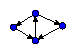
\includegraphics[width=0.85\textwidth]{images/directed-graph.pdf}
						%\caption{Simple Directed graph }
					\end{figure}
				\end{center}
			\end{column}
			\begin{column}{0.45\textwidth}  
				\begin{eqnarray*}
					L &=& D_{out} - A \\
					L &=& \begin{pmatrix}
						2 & -1& 0& -1 \\
						0 & 1& -1 & 0 \\
						-1 & 0& 1 & 0 \\
						0 & 0& -1 & 1 \\
					\end{pmatrix}
				\end{eqnarray*}
			\end{column}
		\end{columns}
		\item To begin with, the laplacian matrix of the directed network is not symmetric. This perhaps brings in a twist in the whole story.
	\end{itemize}
	
\end{frame}

\subsection{Diffusion on networks}
\begin{frame}
	\frametitle{Diffusion on networks}
	
	Diffusion is a process by which information, epidermic, viruses, and any other behaviours spread over networks \cite{newman2010networks}.
	Take a simple undirected connected network. Consider a quantity of substance $\phi_i$ (heat) at each node $i$ at time $t$. The diffusion of heat over the network is given by\\
	\begin{equation}
	\frac{d\phi_i}{dt} = C \sum_j A_{ij}(\phi_j - \phi_i)
	\end{equation} 
	In matrix notation,
	\begin{equation}
	\frac{d\boldsymbol{\phi}}{dt} + C\mathbf{L}\boldsymbol{\phi} = 0, \quad \boldsymbol{\phi}(0) = \boldsymbol{\phi}_0 
	\end{equation}
	whose solution
	\begin{equation}
	\boldsymbol{\phi}(t) = \boldsymbol{\phi}_0~e^{-C\mathbf{L}t}
	\end{equation}  	
\end{frame}

\begin{frame}
	\frametitle{Equilibrium behaviour}
	As time $t$ goes to infinity, the equilibrium state is completely determined by the \textbf{kernel of $\mathbf{L}$}. 
	The quantity of heat $\phi_j(t)$ at any node $j$ at time $t$ is given by
	\begin{equation*}
	\lim_{t \to \infty}\phi_j(t) = \frac{1}{n} \sum_{i = 1}^n \phi_i(0). 
	\end{equation*}
	
	\vspace{1cm}
	\textbf{NOTE:} \\
	%The value at each node at equilibrium is only dependent on the initial quantities of heat as well as the number of nodes $n$. 
	The structure of the network has no influence over the equilibrium value but plays a role in influencing the rate at which diffusion occurs.
\end{frame}

\begin{frame}{Illustration of diffusion over a simple network}
	Suppose we assign to each node heat quantities given by $\phi_0=[2,0,8,0,5,0,0,0,0,0]$ in order node $1$ to $10$. Let $C=1$.
	\begin{figure}[!h]
		%\centering
		\onslide<1->{
			\begin{subfigure}[1]{0.32\textwidth}
				\fbox{\includegraphics[width=0.95\textwidth]{images/img0.png}}
				\caption{$t=0$}
				%\label{stardifn-graph}
		\end{subfigure}}~
		\onslide<2->{\begin{subfigure}[2]{0.32\textwidth}
				\fbox{\includegraphics[width= 0.95\textwidth]{images/img1.png}}
				\caption{$t=1$}
				%\label{stardifn-plot}
		\end{subfigure}}~
		\onslide<3->{\begin{subfigure}[3]{0.32\textwidth}
				\fbox{\includegraphics[width= 0.95\textwidth]{images/img2.png}}
				\caption{$t=2$}
				%\label{stardifn-plot}
		\end{subfigure}}\\
		\onslide<4->{\begin{subfigure}[4]{0.32\textwidth}
				\fbox{\includegraphics[width=0.95\textwidth]{images/img5.png}}
				\caption{$t=5$}
				%\label{regdifn-graph}
		\end{subfigure}}~
		\onslide<5->{\begin{subfigure}[5]{0.32\textwidth}
				\fbox{\includegraphics[width= 0.95\textwidth]{images/img7.png}}
				\caption{$t=7$}
				%\label{stardifn-plot}
		\end{subfigure}}~
		\onslide<6->{\begin{subfigure}[6]{0.32\textwidth}
				\fbox{\includegraphics[width=0.95 \textwidth]{images/img9.png}}
				\caption{$t=9$}
				%\label{regdifn-plot}
		\end{subfigure}}
	\end{figure}
\end{frame}

\begin{frame}{Diffusion on a Lattice}
	
	\begin{figure}[!h]
		%\centering
		\begin{subfigure}[b]{0.25\textwidth}
			\includegraphics[width=\textwidth]{images/anim_0.png}
			%\caption{$x=0, t=0$}
			%\label{gridt0x0}
		\end{subfigure}~
		\begin{subfigure}[b]{0.25\textwidth}
			\includegraphics[width= \textwidth]{images/anim_15.png}
		\end{subfigure}~
		\begin{subfigure}[b]{0.25\textwidth}
			\includegraphics[width= \textwidth]{images/anim_30.png}
		\end{subfigure}~
		\begin{subfigure}[b]{0.25\textwidth}
			\includegraphics[width= \textwidth]{images/anim_45.png}
		\end{subfigure}\\
		\begin{subfigure}[b]{0.25\textwidth}
			\includegraphics[width=\textwidth]{images/anim_50.png}
			%\caption{$x=0, t=0$}
			%\label{gridt0x0}
		\end{subfigure}~
		\begin{subfigure}[b]{0.25\textwidth}
			\includegraphics[width= \textwidth]{images/anim_80.png}
		\end{subfigure}~
		\begin{subfigure}[b]{0.25\textwidth}
			\includegraphics[width= \textwidth]{images/anim_110.png}
		\end{subfigure}~
		\begin{subfigure}[b]{0.25\textwidth}
			\includegraphics[width= \textwidth]{images/anim_145.png}
		\end{subfigure}\\
		\begin{subfigure}[b]{0.25\textwidth}
			\includegraphics[width=\textwidth]{images/anim_200.png}
			%\caption{$x=0, t=0$}
			%\label{gridt0x0}
		\end{subfigure}~
		\begin{subfigure}[b]{0.25\textwidth}
			\includegraphics[width= \textwidth]{images/anim_240.png}
		\end{subfigure}~
		\begin{subfigure}[b]{0.25\textwidth}
			\includegraphics[width= \textwidth]{images/anim_455.png}
		\end{subfigure}~
		\begin{subfigure}[b]{0.25\textwidth}
			\includegraphics[width= \textwidth]{images/anim_500.png}
		\end{subfigure}
		Animation: \url{www.wikipedia.com/laplacian_matrix}
	\end{figure}
\end{frame}

\begin{frame}{Summary}
	\begin{itemize}
		\item Overview of the Network theory approach to the study of complex systems
		\item Representation of Network by the Laplacian Matrix
		\item Applications of the Laplacian Matrix 
		\begin{itemize}
			\item Laplacian centrality for directed weighted networks 
			\item  Possible extension of laplacian centrality to directed networks
			\item Diffusion over networks based on direct interactions between connected nodes
			\item Consideration of non direct interactions in diffusion process on networks
			
		\end{itemize}
	\end{itemize}
	
\end{frame}

%------------------------------------------------

%\begin{frame}
%\frametitle{References}
%\footnotesize{
%\begin{thebibliography}{99} % Beamer does not support BibTeX so references must be inserted manually as below
%\bibitem[Smith, 2012]{p1} John Smith (2012)
%\newblock Title of the publication
%\newblock \emph{Journal Name} 12(3), 45 -- 678.
%\end{thebibliography}
%}
%\end{frame}

%\begin{frame}
%	\movie[height = 0.6\textwidth, width = 0.8\textwidth, poster, showcontrols]{}{movie.mp4} 
%\end{frame}

%\begin{frame}[allowframebreaks]
%	\frametitle{References}
%	
%	\nocite{*}
%	\bibliographystyle{abbrv}
%	\bibliography{bmsreferences}
%\end{frame}

%------------------------------------------------
{\2
\begin{frame}[noframenumbering, plain]
	\begin{center}
		\Huge{\textbf{Merci}}
	\end{center}
\end{frame}}

%-------------------------
\end{document}